\cotefile{72}
\scanpage{35}
\margin{?}D'ailleurs, si $N=2$, $\exists 1$ \deleted{quadrique}\inserted{conique} $Q\subset X$ \unsure{invariante} par $\varphi^{+}$, et elle est \deleted{\unsure{--}} invariante par $\varphi$.

[Peut-être faut-il se donner au préalable \deleted{forme quadratique}\inserted{\unsure{hyp.\ qu.\ \unsure{entière|encore|conique} lisse|hyp.\ conique lisse}} \unsure{invariante|invariantes} \ldots{}]
% archive sheet number: 34
\scanpage{36}
Supposons les $\beta_i\inserted{=\alpha_i+2}$ inv.

\[
\begin{aligned}
\text{forme sur }&\unsure{\mathrm{G}|\mathcal G|Q|\mathcal Q|\mathcal O}(a_{i-1},\unsure{a_i|\tau_i},a_{i+1})\ \text{lisse}\iff\alpha_{i-1}+\alpha_i\quad\text{inv.}\\
\text{forme sur }&\mathrm{G}(a_{i-1},a_i)\ \text{lisse}\iff 2-\alpha_{i-1}\quad\text{inv.}\\
\text{\rule{2.6cm}{0.35pt} }&\mathrm{G}(a_i,a_{i+1})\ \text{lisse}\iff 2-\alpha_i\quad\text{inv.}
\end{aligned}
\]

\diagram{\begin{tikzcd}[ampersand replacement=\&,column sep=large,row sep=0pt]
\deleted{\unsure{\alpha_i|\text{Ex.}}} \& a_{i-1}\arrow[r,dash,to path={-- ++(0,-.65em) -| (\tikztotarget)},swap,"{2-\alpha_{i-1}}"] \& a_i\arrow[r,dash,to path={-- ++(0,-.65em) -| (\tikztotarget)},swap,"{2-\alpha_i}"] \& a_{i+1}
\end{tikzcd}}

\[
\begin{aligned}
\alpha_{i}&\ne 2\qquad\text{\unsure{l'une|hyp.|cas} des val. propres }1\\
\alpha_{i-1}&\ne 2
\end{aligned}
\]

\deleted{\unsure{Donc}} Si
\[
\left.\begin{aligned}
&\beta_0,\ldots,\beta_{n-1}\quad\text{inv.}\\
&2(\alpha_{i-1}+\alpha_i)\quad\text{inv.}\ \inserted{\boxed{\text{donc car. }\ne2\,!}}\\
&\alpha_{i-1}-2,\ \alpha_i-2\quad\text{inv}
\end{aligned}\right\}
\]
\margin{\unsure{Sur $i$|pour} \quad $1\le i\le n-1$}alors $\tau_i$ se reconstruit à partir des $\underset{\substack{\Vert\\ \tau_{i-1}\tau_i}}{\rho_{i-1}},\underset{\substack{\Vert\\ \tau_i\tau_{i+1}}}{\rho_i}$ donc aussi $\tau_{i-1}=\rho_{i-1}\tau_i$, $\tau_{i+1}=\tau_i\rho_i$.

\margin{\uline{dans $V,f$} ou $C=\mathbb{P}(V),Q$ $(n\geq2)$}
% slanted
$\tau_i={}$\deleted{sym} réflexion associée à la direction

\[
\begin{aligned}
\left(
\underbrace{V^{\rho_{i-1}}}_{\substack{\deleted{\unsure{=}}\Vert\\\{a_{i-1},a_i\}^{\perp}}}
+\underbrace{V^{\rho_i}}_{\substack{\Vert\\\{a_i,a_{i+1}\}^{\perp}}}
\right)^{\perp}
&=\{a_{i-1},a_i\}^{\perp\perp}\cap\{a_i,a_{i+1}\}^{\perp\perp}\\
&=\mathrm{G}(a_{i-1},a_i)\cap\mathrm{G}(a_i,a_{i+1})
\end{aligned}
\]

\[
\alpha_i=\frac{(a_i,a_{i+1})^2}{f(a_i)f(a_{i+1})}=4\cos^2\theta_i\ \deleted{\unsure{\cos 2|\alpha_i\cos 2}}
\]

\[
\beta_i=\alpha_i+2=2\bigl(\underbrace{2\cos^{2}\theta_i+1}_{\deleted{\unsure{2}}\cos 2\theta_i}\bigr)=4\cos2\theta_i
\]
% archive sheet number: 35
\scanpage{37}
\[
\deleted{\unsure{G}}U_{\rho}\simeq\operatorname{Aut}\bigl(\deleted{\unsure{E}}X,(\tau_{\unsure{*|\bullet|i}})\bigr)
\]
% archive sheet number: 36
\scanpage{38}
Soit $\rho\in\Gamma(S,\mathcal O_S)$, $U_\rho\subset\mathbb E^{1}_{S}$ formé des $\lambda$ tels que $1+\lambda\rho$ inversible i.e.

\[
U_\rho=\underline{\operatorname{Spec}}\ \mathcal O_S[T]_{(1+\rho T)}
\]

prenons la multiplication

\[
(\lambda\mathbin{\underset{\rho}{*}}\lambda'=\lambda+\lambda'+\lambda\lambda'\rho
\]

de sorte que $U_\rho$ est un schéma en groupes\inserted{(lisse comm. \unsure{de rel.|de dim.\ rel.} 1)}, et

\[
\begin{aligned}
\lambda&\mapsto 1+\lambda\rho\\
U_\rho&\longrightarrow G_m
\end{aligned}
\]

est un hom de groupes, qui est un iso. sss $\rho$ inversible.

Considérons un hyperpolyèdre régulier \unsure{paramétré|ponctué|pseudo-} épinglé sur $S$, de dim. $n$\inserted{(\unsure{ou 3|ou 1|tous|conv.})}, correspondant \unsure{à|:|;} des invariants $\mu_i$ $(0\leq i\leq n)$ et $\beta_i$ $(0\leq i\leq n-1)$ [avec $\mu_i+1$ inv. $0\leq i\leq n$). Soit \deleted{$\rho=\unsure{\mathbb L|L}_{n+1}(\mu_0,\lambda_0,\ldots,\lambda_{n-1},\mu_n)$}

\[
\unsure{=}\qquad \rho=\mathbb L_{n+1}(\mu_0,\lambda_0,\ldots,\lambda_{n-1},\mu_n)=\langle\pi,\pi'\rangle
\]
% archive sheet number: 37
\scanpage{39}
Donc $U_\rho$ opère \inserted{\unsure{fidèlt|fidèlem.|fidèlement}} sur $\unsure{E|\mathcal E},E'$ par

\[
\left\{\begin{aligned}
u_\lambda^E &=\mathrm{id}+\lambda\pi'\otimes\pi\\
u_\lambda^{E'}&=\mathrm{id}+\lambda\pi'\otimes\pi
\end{aligned}\right.
\]

(\unsure{représentations|opérations} \deleted{\unsure{contragrédientes}}\inserted{transposées} l'une de l'autre) Comme $\pi,\pi'$ \unsure{invariants|invariantes} sous les $\tau_i$, \deleted{\unsure{donc pour|donc aussi}} sous les $\varphi^E(s)$, $\varphi_{\unsure{*|s}}^{E'}(s)$ $(s\in G_n)$, on trouve

\[
\begin{aligned}
\unsure{\alpha_2|\alpha'|(*)}\quad U_\rho&\longrightarrow\underline{\operatorname{Aut}}(E,\varphi^E)\\
\alpha\quad U_\rho&\longrightarrow\underline{\operatorname{Aut}}(X,\varphi^X)
\end{aligned}
\]

et de $=$ avec $E'$. On obtient en fait, en utilisant les scalaires

\diagram{\begin{tikzcd}[ampersand replacement=\&,column sep=small,row sep=small]
(\unsure{\alpha\alpha|\alpha *|**}) \& G_m\times U_\rho\arrow[rr]\&\&\operatorname{Aut}(E,\varphi^E)\\
\&\&G_m\arrow[ul,hook']\arrow[ur,swap,"\text{opère par homothéties}"]\&
\end{tikzcd}}

dont $\alpha$ est déduit en passant au quotient. On trouve

\uline{Th\unsure{m|me}} $\alpha$ et $(\alpha\alpha)$ sont des iso.

De plus, si $D_0=(H_1\cap\cdots\cap H_n)$, $D_0^{**}=D_0\setminus\{c,d\}$, où $\unsure{\exists|\,|\{}d=D_0\cap C$ (qui est une section de $X$ sur $S$) \unsure{.|:} on a que
% archive sheet number: 38
\scanpage{40}
$U_\rho$ opère (sans \unsure{mérite|unité}!) sur $D_0$ et $D_0^{**}$, et que $D_0^{**}$ est un \uline{torseur} sous $U_\rho$\unsure{,} (trivialisé par $s_0\ldots$)

\begin{center}\rule{2.1cm}{0.35pt}\end{center}

Supposons maintenant les $\mu_i=2$ de sorte qu'on a une forme quadratique \uline{inv.} canonique $f$ sur $\unsure{E|\mathcal E}$, unique par la condition

\[
f(a_{-1})=0,\qquad f(e_0)=1,
\]

\deleted{\unsure{Je di|Jx de}} d'où $Q\subset X=\mathbb P^{n}(E)$.

On sait que la ps \unsure{réfle|réfl.} $\mathrm{id}+\underbrace{\lambda\pi'\otimes\pi}_{\pi'\otimes\lambda\pi}$ est \deleted{\unsure{une}} \unsure{orthogonal|orthogonale} sss \deleted{\unsure{si}}l'opération corr. dans $X$ conserve $Q$, et ceci signifie que

\[
\begin{aligned}
&\deleted{\unsure{\lambda}}\unsure{f(\deleted{\unsure{\psi f|\psi|\varphi}}\lambda\pi)|f(\pi)}\pi'+\psi(\lambda\pi)=0\quad\text{i.e.}\\
&\lambda\bigl[\lambda\underbrace{f(\pi)}_{-\widetilde\sigma\widetilde\rho}\pi'+\underbrace{\psi(\pi)}_{-\sigma\pi'}\bigr]=0\qquad\text{i.e.}\\[-2pt]
&\hspace{1.5em}\deleted{\unsure{\lambda f\pi'+{}}}
\end{aligned}
\]

\[
\lambda(\sigma+\lambda\widetilde\sigma\widetilde\rho)=0
\tag*{$(**)$}
\]
% archive sheet number: 39
\scanpage{41}
1) Cas $n$ pair, $\rho=2\widetilde\rho$, $\sigma=\widetilde\sigma$, l'équation s'écrit

\[
\lambda\sigma(1+\deleted{\unsure{2}}\lambda\widetilde\rho)=0
\]

Si $\sigma$ \deleted{\unsure{est}}\inserted{et $\widetilde\rho$} inversibles, la seule solution \uline{inversible} (\inserted{i.e.} correspondant à une section de $U_\rho$ partout $\ne 1$) est donnée par

\[
\lambda=-\frac{1}{\deleted{\unsure{2|4}}\widetilde\rho}\qquad
\text{d'où}\qquad
\underbrace{u=\mathrm{id}-\frac{1}{\deleted{\unsure{2|4}}\widetilde\rho}\pi'\otimes\pi}_{\text{\uline{antipodisme}}}
\]

\deleted{Si \uline{$\sigma=0$} $\unsure{G_\rho|U_\rho|\mathcal U_\rho}$ invarie $f$, \unsure{ou|ce|on} ce qui revient au $=$,}

D'autre part, conditions équivalentes

\diagram{\begin{tikzcd}[ampersand replacement=\&,column sep=0pt,row sep=small]
{} \& {}\\
\mathrm b)\ \&U_\rho\ \text{invarie }f^E\\
\mathrm c)\ \&U_\rho\ \text{invarie } Q_X^{\deleted{\unsure{E|X}}}\\
\mathrm a)\arrow[uuu,bend left=75]\ \&\sigma=0
\end{tikzcd}}

Enfin, si $\widetilde\rho=0$, \deleted{deux}\inserted{ces} conditions \unsure{équivalent|équivalentes} encore à la suivante

\deleted{a) $\sigma=0$}

d) $\exists$ loc. section \deleted{\unsure{divise}} de $U_\rho$ partout $\ne1$ qui invarie $f^E$. \deleted{(ou, ce qui revient au $=$)}\inserted{(ou aussi, $Q_X$)}.
% archive sheet number: 40
\scanpage{42}
\unsure{2)|2°)|$\beta$)} Cas $n$ impair $\rho=\widetilde\rho$, $\sigma=2\widetilde\sigma$, l'équation s'écrit

\[
\lambda\widetilde\sigma(2+\lambda\rho)=0
\]

Donc si $\sigma\inserted{\unsure{\sigma}}(=2\widetilde\sigma)$ et $\rho\inserted{(=\widetilde\rho)}$ inv., \deleted{la seule} $\exists\unsure{1|!}$ section $u$ de $U_\rho$, partout $\ne1$, \deleted{telle} qui invarie $f$, ou ce qui revient au $=$, qui invarie $Q$ -- savoir
\margin{\uline{NB} Si $\widetilde\sigma$ inv. et non $\sigma$ (p. \unsure{x.|ex.} en car. 2) on a \unsure{quand même} unique solution en $\lambda$, savoir $\lambda=-\dfrac{2}{\rho}$, mais celle-ci peut être nulle en certains pts. \unsure{Donner|Donnons|Donc} énoncé commun aux cas 1°) et \unsure{2°)} \unsure{en termes de}  $\boxed{\sigma\widetilde\rho\ \text{inversibles}}$}
% slanted

\[
\underbrace{u=\mathrm{id}\unsure{-|+}\frac{2}{\rho}\pi'\otimes\pi}_{\text{antipodisme}}
\]

D'autre part, conditions équiv.\deleted{\unsure{alentes}}

\deleted{\unsure{si}} a) $2\widetilde\sigma=\sigma=0$ et $\widetilde\sigma\rho\inserted{(=\unsure{\widetilde\sigma\widetilde\rho|\sigma\rho})}=0$.

[\uline{NB} si 2 inv., celà équivaut à $\sigma=0$; si $\unsure{2\cdot1_S|2\,1_S}=0$, celà équivaut à $\widetilde\sigma\rho=0$]

b) $U_\rho$ invarie $f^E$

\margin{\unsure{itou|i.e.}}
% slanted
c) $U_\rho$ \rule{1.6cm}{0.35pt} $Q_X$

Si \deleted{de plus} $\rho=0$, ces conditions équivalent aussi à :

d) $\exists$ \inserted{loc.} section de $U_\rho$ partout $\ne1$ qui invarie $f^E$ (ou encore, $Q_X$)
% archive sheet number: 41
\scanpage{43}
[\uline{Ex} $n=1$, $\rho=4-\beta=2-\alpha$, $\sigma=\deleted{\unsure{\alpha}}\;2$, $\widetilde\sigma=1$. Donc

\deleted{Par} 1°) si $\deleted{\unsure{2}}\rho$ inv. \inserted{i.e. $U_\rho\simeq G_m$,} alors $\exists\unsure{1|!}\ u\in U_{\rho=2-\alpha}$ partout $\ne1$, telle que $u$ invarie $f^E$ (ou ce qui revient au $=$, \deleted{$Q_X$} la conique $Q_X$) savoir l'antipodisme, qui est l'unique section $u$ telle que $u^2=1$, $u_s\ne1$ $\forall s\in S$.

2°) Conditions équivalentes

a) $\rho=0$ et \deleted{\unsure{car.|car}} $S$ de car 2 $(2.1_S=0)$

b) $U_\rho$ invarie $f^E$

c) $U_\rho$ \rule{1.5cm}{0.35pt} $Q_X$

d) $\rho=0$ et $\exists$ loc. section partout $\ne1$, qui invarie $f^E$ (ou encore, $Q_X$).]

\begin{center}\rule{4cm}{0.35pt}\end{center}

\uline{Proposition} 1) Si $\sigma\widetilde\rho$ inversible, $\exists1$ section $u$ de $U_\rho$, partout $\ne1$, qui invarie $f^E$ i.e. $Q_X$, savoir l'antipodisme.

2) Conditions équivalentes

a) $\sigma=0$ et $\widetilde\sigma\widetilde\rho=0$ (cette dernière condition conséquence de la première si $n$ pair ou 2 inv)

b) $U_\rho$ invarie $f^{\deleted{\unsure{E|X}}E}$

c) $U_\rho$ invarie $Q_X$

\margin{\unsure{?|2}}d) (\uuline{si $\widetilde\sigma\widetilde\rho=0$}) $\exists$ loc. section de $U_\rho$ partout $\ne1$, qui invarie $f^E$ (\uline{ou} $Q_X$)
% archive sheet number: 42
\scanpage{44}
Calculs de discriminants etc.
% archive sheet number: 43
\scanpage{45}
\[
\left\{\begin{aligned}
f(s_i)&=0\\
\varphi(s_i,s_j)&=-(\alpha_0+2)\cdots(\alpha_{i-1}+2)\qquad 0\le i<j\le n+1
\end{aligned}\right.
\]

$f$ caractérisée par les conditions

a) $f$ inv. par les $\tau_i$

b) $f(s_0)=0$ ($\iff f$ nulle sur les sommets \unsure{génér.|gén.|fixés} \unsure{du|au} $\Pi$)

c) $f(a_0)=1$ ($\iff$ \deleted{\unsure{2}} vecteurs arêtes sont unitaires)

\[
\begin{aligned}
f(a_i)&=(\alpha_0+2)\cdots(\alpha_{i-1}+2) &&0\le i\le n\\
\varphi(a_i,a_j)&=0 &&0\le i<j\le n,\ i\unsure{,|{}}j\ \text{non conséc.}\\
\varphi(a_i,a_{i+1})&=-(\alpha_0+2)\cdots(\alpha_i+2)\\
\varphi(s_0,a_i)&=0 &&1\le i\le n\\
\varphi(s_0,a_0)&=-1
\end{aligned}
\]

\[
\left\{\begin{aligned}
\varphi(s_0,s_1)&=\varphi(s_0,a_1)\inserted{=\varphi(s_0,a_0)}=-1\\
\varphi(s_1,a_0)&=f(a_0)=1\\
\tau_0&\ \text{str. orth.}
\end{aligned}\right.
\]

\[
\begin{aligned}
\varphi(s_j,a_i)&=0 &&0\le j<i\le n,\quad\deleted{\unsure{i\geq j+1}}\\
\varphi(s_j,a_{j\deleted{\unsure{+1}}})&=-(\alpha_0+2)\cdots(\alpha_{j-1}+2)&&0\le j\le n\\
\varphi(s_j,a_{j-1})&=+(\alpha_0+2)\cdots(\alpha_{j-2}+2)&&1\le j\le n+1\\
\varphi(s_j,a_i)&=0&&0\le i<j-1\le n
\end{aligned}
\]

\deleted{$\alpha_i+2$ inversibles $(0\le i\le n-1)\iff\tau_{\unsure{i}}$}

\[
\begin{aligned}
\tau_i\ \text{réflexion strictement orthogonale}&\iff(\alpha_0+2),\ldots,(\alpha_{i-1}+2)\in k^{*}\\
(\tau_i\ \text{str. orth. }\ \forall 0\le i\le n)&\iff(\alpha_i+2)\in k^{*}\quad\forall 0\le i\le n-1
\end{aligned}
\]
% archive sheet number: 44
\scanpage{46}
\[
\left\{\begin{aligned}
f(s_i)&=0 &\varphi(s_i,s_i)&=0\\
\varphi(s_i,s_j)&=-(\alpha_0+2)\cdots(\alpha_{i-1}+2)&0&\le i<j\le n+1
\end{aligned}\right.
\]

\deleted{$f(\unsure{s_0|a_0})$} \deleted{$f(\unsure{a_0})=$}
\[
\left\{\begin{aligned}
f(a_{-1})&=0\inserted{=c_{-2}},\quad f(a_i)=(\alpha_0+2)\cdots(\alpha_{i-1}+2)=c_{i-1}\\
\varphi(a_i,a_j)&=0\quad -1\le i\deleted{\unsure{\le}}<j\le n\qquad\deleted{\unsure{i,j\ \text{non successifs}}}\\
\varphi(a_i,a_{i+1})&=-(\alpha_0+2)\cdots(\alpha_i+2)=\deleted{\unsure{c_i}}-c_i\quad -1\le i\le n-1
\end{aligned}\right.
\]
\margin{-- Attention au chgt de \unsure{notations|notation}}

\[
\begin{aligned}
&0\le i\le n\\
&\deleted{\unsure{0\le i\le n}}\quad\varphi(a_i,a_i)=2f(a_i)=2(\alpha_0+2)\cdots(\alpha_{i-1}+2)\\
&0\le i\le n\\
&i,j\ \text{non consécutifs}
\end{aligned}
\]

Matrice de $f$ p.r. à la base $(a_i)_{-1\le i\le n}$

\[
\deleted{\left(\begin{array}{ccccc}0&-1&&&\\-1&\unsure{2}&\unsure{-c_0}&&\\&\unsure{0}&c_0&&\\&&&c_1&\\&&&&c_{n-1}\end{array}\right)}
\qquad f=\left(\begin{array}{ccccccccc}
0&-1&&&&&&&\\
-1&\unsure{2|1}&-c_0&&&&&&\\
&-c_0&2c_0&-c_1&&&&&\\
&&-c_1&2c_1&-c_2&&&&\\
&&&-c_2&2c_2&-c_3&&&\\
&&&&-c_3&2c_3&&&\\
\text{--}&&&&&&\ddots&&\\
&&&&&&&2c_{n-2}&-c_{n-1}\\
&&&&&&&-c_{n-1}&2c_{n-1}
\end{array}\right)
\]

\deleted{$\det\unsure{M_{r}f|M_f}$}
\[
\begin{aligned}
\delta(f)&=\det\left(\begin{array}{ccccc}
-1&-c_0&0&0&\\
0&2c_0&-c_1&0&\\
\big|&\unsure{-}c_1&2c_1&-c_2&\\
\big|&0&\unsure{-}c_2&2c_2&\big|\\
0&\big|&\big|&-c_3&\ddots\\
0&0&0&\text{--}&2c_{n-1}
\end{array}\right)
=-1\det\left(\begin{array}{ccccc}
2c_0&-c_1&&0&\\
-c_1&2c_1&-c_2&&\\
&-c_2&\ddots&\ddots&\\
0&\ddots&&&-c_{n-1}\\
&&&-c_{n-1}&2c_{n-1}
\end{array}\right)\\
&\qquad{}+\underbrace{c_0\det\left(\begin{array}{cccc}0&&&\\0&-&-&\\\big|&&-&-\\0&\text{---}&&\end{array}\right)}_{0}
\end{aligned}
\]

\[
\det\left(\begin{array}{ccccccc}
2c_{-1}&-c_0&0&0&\cdots&&0\\
-c_0&2c_0&-c_1&&&&\vdots\\
0&-c_1&2c_1&&&&\big|\\
\vdots&&&\ddots&&&0\\
\big|&&&&\ddots&&-c_{n-1}\\
0&\text{---}&&&0&-c_{n-1}&\deleted{\unsure{2}}2c_{n-1}
\end{array}\right)
=F_{n+1}(\underbrace{c_{-1},\ldots,c_{n-1}}_{n+1\ \text{arguments}})
\]

\[
\begin{aligned}
-\delta(f)&=\unsure{a|{}}F_n(c_0,\ldots,c_{n-1})=2c_0F_{n-1}(c_1,\ldots,c_{n-1})+c_1\det
\left(\begin{array}{ccccc}
-c_1&-c_2&0&0&\\
0&2c_2&-c_3&0&\\
\big|&-c_3&2c_3&-c_4&\\
\big|&0&-c_4&2c_4&\\
&\big|&0&-c_5&\\
0&0&\vdots&\big|&\\
&&0&\big|&c_{n-1}
\end{array}\right)\\
&=2c_0\inserted{F_{n-1}(c_1,\ldots,c_{n-1})}\unsure{-|+}c_1^2F_{n-2}(c_2,\ldots,c_{n-1})
\end{aligned}
\]

\[
0\to1\to2\to3\ \ldots\to n-1\to0\qquad\text{permutation \uline{circulaire $u$ ou $u^{-1}$}}
\]

\[
\begin{aligned}
F_1(c_0)&=2c_0\qquad F_2(c_0,c_1)=4c_0c_1\unsure{-|+}c_1^2\\
&\hspace{9em}=c_1(4c_0-c_1)\\
F_3(c_0,c_1,c_2)&=2c_0(4c_1c_2-c_2^2)-2c_1^2c_2\\
&\deleted{=8c_0c_1c_2}\\
&=2c_2(4c_0c_1-\deleted{\unsure{2}}c_0c_2-\deleted{\unsure{2}}c_1^2)
\end{aligned}
\]
% archive sheet number: 45
\scanpage{47}
\[
\det\bigl((c_{ij})_{1\le i,j\le n}\bigr)\overset{?}{=}
\qquad c_{ij}=0\quad\text{si } i\ne j,\ i,j\ \text{non consécutifs}
\]

\[
\sum_{\sigma\in\unsure{\mathfrak S_n|\mathcal S_n}}\varepsilon_\sigma
\underbrace{\prod_{i=1}^{n} c_{i,\sigma(i)}}_{\phantom{c_{ii}}}
\quad\unsure{\text{''}|\Vert}\quad\unsure{*}
\]
nul, sauf si $\sigma$ est tel que $\overbrace{\forall i\in[1,n],\ \sigma i\in\{i-1,i,i+1\}}^{\sigma\ \text{admissible}}$

Supposons $n\ge\unsure{3|2}$, alors tt cycle de $\sigma$ est de longueur 1 ou 2 et les cycles de long. 2 sont formés d'entiers consécutifs, donc $\unsure{\tau|\sigma}$ est de la forme

\diagram{\begin{tikzcd}[ampersand replacement=\&,column sep=small]
i-2\arrow[r,dash]\arrow[r,bend right,dash] \& i-1\arrow[r,dash]\arrow[r,bend right,dash] \& i
\end{tikzcd}}

\[
\unsure{\overline{\sigma}|\sigma|\tau}_{i_1}\overline{\sigma}_{i_2}\ldots\overline{\sigma}_{i_p}
\qquad 1\le i_1<i_2\ldots<i_p\le n-1
\]
($\overline{\sigma}_i$ est la transposition de $i,i+1$) où $i_1\ i_2\ldots i_p$ sont \deleted{\unsure{des entiers}} entiers non consécutifs.

\[
\deleted{\sum_{\substack{i_1\,i_2\ldots i_p\\\text{suites str. cr.}\\\text{d'entiers}}}}
\quad
\underbrace{1+\alpha_{\unsure{1|0}}}_{i_1}\quad
\underbrace{\deleted{\unsure{i_1+}}3+\alpha_{\unsure{1|0}}+\alpha_2}_{i_2}\quad
\underbrace{i_1+5+\alpha_0+\alpha_{\unsure{2|1}}+\alpha_3}_{i_3}\quad\ldots\quad
\underbrace{\deleted{\unsure{i_1+}}(2\unsure{(p-1)|p-1})+\alpha_0\ldots+\alpha_p}_{i_p}
\]

\[
\begin{aligned}
&\deleted{1\le i_1\qquad i'_1+\alpha_1+\cdots+\alpha_{p-1}\le{}}\\
&\alpha_i\in\mathbb N\qquad \alpha_0+\cdots+\alpha_{p-1}\le n-2p
\end{aligned}
\]

\[
\begin{aligned}
&\sum_{1\le p\le[n/2]}(-1)^p
\sum_{\substack{(\alpha_{\unsure{1|0}},\ldots,\alpha_p)\in\mathbb N^p\\\sum\alpha_i=n-2p}}
\deleted{\unsure{\prod_i}}
\prod_{\substack{1\le i\le n\\\text{non de la}\\\text{forme}\\
i\left\{\begin{smallmatrix}(2r-1)+(\alpha_{\unsure{1|0|p}}\,\ldots+\alpha_r)\\
2r+(\alpha_{\unsure{1|0|p}}\,\ldots+\alpha_r)\end{smallmatrix}\right.\\1\le r\le p}}
c_{ii}\\
&\quad\prod_{1\le r\le p}
\left(\begin{aligned}
&c_{2r-1+(\alpha_1+\cdots+\alpha_r),\,2r+(\alpha_1+\cdots+\alpha_r)}\\[-2pt]
&c_{2r+(\alpha_1+\cdots+\alpha_r),\,2r-1+(\alpha_1\ldots+\alpha_r)}
\end{aligned}\right)
\end{aligned}
\]

Supposons matrice \uline{symétrique}, et $c_{i\,i+1}=-c_{i+1}$ \quad $c_{ii}=2c_i$

On trouve

\[
\det\bigl((c_{ij})_{1\le i,j\le n}\bigr)=
\sum_{1\le p\le[n/2]}(-1)^p2^{\inserted{n-2p}}
\sum_{\substack{\alpha_*\in\mathbb N^p\\\alpha_1+\cdots+\alpha_p\le n-2p}}
\prod_i c_i\prod_{1\le\unsure{t|r}\le p}
(c_{2r+\alpha_1+\cdots+\alpha_r})^2
\]

\figure{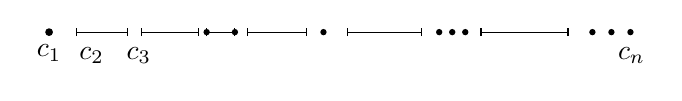
\begin{tikzpicture}[x=.69cm,y=.55cm]
\fill (0,0) circle (1.4pt);
\node[below] at (0,-.07) {$c_1$};
\foreach \a/\b in {.5/1.45,1.7/2.75,2.9/3.42,3.65/4.74,5.5/6.85,7.95/9.55}{
\draw (\a,-.09)--(\a,.09) (\a,0)--(\b,0) (\b,-.09)--(\b,.09);}
\node[below] at (.78,-.12) {$c_2$}; \node[below] at (1.65,-.12) {$c_3$};
\foreach \a in {2.9,3.42,5.05,7.18,7.42,7.66,10,10.35,10.7}{\fill (\a,0) circle (1.15pt);}
\node[below] at (10.72,-.12) {$c_n$};
\end{tikzpicture}}

\unsure{$c$|(|$C$}
% archive sheet number: 46
\scanpage{48}
\[
\langle a_i,a'_j\rangle=
\begin{cases}
0&\text{si } i\ne j,\ i\text{ et }j\text{ non consécutifs}\\
1&\text{si \deleted{\unsure{voisins}} }i=j-1\\
\deleted{\unsure{+|2\lambda_j}}\lambda_j-1&\text{si \deleted{\unsure{égal}} }i=j\\
-\lambda_j+1+\alpha_j&\deleted{\unsure{\text{si $j$ voisin}}}\quad i=j+1
\end{cases}
\]

\[
\begin{aligned}
a_i&=s_{i+1}-s_i\\
a'_j&=s_j^*+\lambda_j s_{j+1}^*+(1+\alpha_j)(s_{j+2}^* \ldots+s_{n+1}^*)\qquad 0\le j\le n\\
a'_n&=
\end{aligned}
\]

\[
\deleted{\boxed{\begin{aligned}\psi(a_{-1})&=-a_0^*\\\psi(a_n)&=-c_{n-2}a_{n-1}^*+2c_{n-1}a_n^*\end{aligned}}}
\]

\[
\left\{\begin{aligned}
a'_j&=a_{j-1}^*+\underbrace{(\lambda_j-1)}_{-2\ \text{si }\lambda_j=-1}a_j^*+
\underbrace{(1-\lambda_j+\alpha_j)}_{\beta_j=2+\alpha_j\ \text{si }\lambda_j=-1}a_{j+1}^*
\quad\deleted{\unsure{*}}0\le j\le n-1\\
a'_n&=a_{n-1}^*+(\lambda_n-1)a_n^*\deleted{\unsure{+}}\\
\pi&=a_{-1}^*\\
s_j&=a_{-1}+\ldots+a_{j-1}\qquad0\le j\le n+1
\end{aligned}\right.
\]

\[
\begin{aligned}
f(a_i)\deleted{\unsure{\varphi(}}a'_i\unsure{1|)|{}}+\psi(\unsure{a_i|a'_i})&=0\\
f\bigl(\sum_{-1}^{n}\zeta_i a_i\bigr)&=\sum_{i=0}^{n}c_{i-1}\zeta_i^2\\
&\unsure{-|+}\sum_{-1\le i\deleted{\unsure{<}}\le n-1}c_i\zeta_i\zeta_{i+1}
\end{aligned}
\]

\deleted{$\psi(a_i)=-c_{i-1}a_{i-1}^*+2c_{i-1}a_i^*-\unsure{c_2|c_i}a_{i+1}^*$} \quad $0\le i\le n-1$

$\longleftrightarrow$ On pose \deleted{\unsure{rappelons|rappelons que}} $c_{-1}=1$
\[
\begin{aligned}
c_0&=(\alpha_0+2),\ldots\quad c_i=(2+\alpha_0)\cdots(2+\alpha_i)\\
&0\le i\le n\hspace{6em}0\le i\le n-1\\
c_n&=c_{n+1}=0
\end{aligned}
\]

Coordonnées \deleted{projectives} de $c$, orth. aux $a'_i$ (on fait $\lambda_i=-1$ pour $0\le i\le n$)

\[
\begin{aligned}
c'&=\sum_{-1}^{n}\zeta_i a_i\quad(\zeta_n=1)\\
\zeta_{n-1}-2\zeta_n&=0\qquad\deleted{\unsure{\zeta_{n-1}=2|\xi_{n-1}=2}}\quad\boxed{\zeta_n=1,\ \zeta_{n-1}=2}\\
\zeta_{n-2}-2\zeta_{n-1}+(\alpha_{n-1}+2)\zeta_n&=0\qquad\boxed{\zeta_{n-2}=-(\alpha_{n-1}-2)}\\
\zeta_{n-3}\underbrace{-2\zeta_{n-2}+(\alpha_{n-2}+2)\zeta_{n-1}}_{\substack{2(\alpha_{n-1}-2)+(\alpha_{n-2}+2)2\\=2(\alpha_{n-1}+\alpha_{n-2})}}&=0
\qquad\boxed{\zeta_{n-3}=-2(\alpha_{n-1}+\alpha_{n-2}}\\
\zeta_{n-4}\underbrace{\unsure{-|+}2\zeta_{n-3}+(\alpha_{n-3}+2)\zeta_{n-2}}_{4(\alpha_{n-1}+\alpha_{n-2})\unsure{-|+}(\alpha_{n-3}+2)(\alpha_{n-1}-2)}&=0
\end{aligned}
\]

\[
\boxed{\begin{aligned}
\zeta_{n-4}&=\deleted{\unsure{\alpha_{n-1}}(\alpha_{n-3}+2)+4\alpha_{n-2}+4+{}}\\
&-4-2(\alpha_{n-1}+2\alpha_{n-2}+\alpha_{n-3})\\
&\quad+\alpha_{n-1}\alpha_{n-3}
\end{aligned}}
\]

\[
\begin{aligned}
&2\underline{\alpha_{n-1}}+4\underline{\alpha_{n-2}}+\underline{4}-\underline{\alpha_{n-1}\alpha_{n-3}}+2\underline{\alpha_{n-3}}\\
&\zeta_{n-5}=\ldots
\end{aligned}
\]

\[
\begin{aligned}
\pi&=a_{-1}^*\\
\pi(c')&=\underline{\rho}(\underbrace{\alpha_0,\ldots,\alpha_{n-1}}_{A})=\rho=\zeta_{-1}\\
&\underline{\rho}\in\mathbb Z[A_0,\ldots,A_{n-1}]\\
c&=\frac{c'}{\rho}\\
f(c')&=\underbrace{\underline\sigma(\alpha_0,\ldots,\alpha_{n-1})}_{\underline\sigma\in\mathbb Z[A_0,\ldots,A_{n-1}]}=\sigma\\
f(c)&=\sigma/\rho^2\qquad 2\sigma=-\zeta_0\zeta_{-1}=-\rho\zeta_0
\end{aligned}
\]

\[
\begin{aligned}
2f(c')&=\langle c',\psi(c')\rangle\overset{?}{=}\\
&\deleted{\psi(c')=\inserted{\lambda\pi={}}\lambda a_{-1}^*\qquad\lambda=\langle a_{-1},\psi(c')\rangle=\varphi(a_{-1},c')}\\
\langle a_i,\psi(c')\rangle&=\varphi(a_i,c')=\langle c',\underbrace{\psi(a_i)}_{-f(a_i)a'_i}\rangle
=\deleted{\unsure{-f(a_i)}}\qquad/\,\text{si }0\le i\le n\\
&=-f(a_i)\langle c',a'_i\rangle=0\ \deleted{\text{si }0\le i\le n}\\
\langle a_{-1},\psi(c')\rangle&=\langle c',\underbrace{\psi(a_{-1})}_{-a_0^*}\rangle=-\deleted{\unsure{\zeta_{-1}}}\zeta_0=\\
\psi(c')&=-\zeta_0 a_{-1}^*\\
&\qquad 2f(c')=\langle c',-\zeta_0a_{-1}^*\rangle=-\zeta_0\zeta_{-1}
\end{aligned}
\]
% archive sheet number: 47
\scanpage{49}
\inserted{$\Delta_{n+2}(0,1,c_0,\ldots,c_{n-1})$}
\[
\begin{aligned}
\deleted{\unsure{\det}}\ \Delta_n(\underbrace{c_0,\ldots,c_{n-1}}_{n\ \text{arg.}})
&=\unsure{-|{}}\det\left(\begin{array}{cccccccc}
0&-1&0&0&0&0&\cdots&0\\
-1&2&-c_0&0&0&0&\cdots&0\\
0&-c_0&2c_0&-c_1&0&0&\cdots&\vdots\\
0&0&-c_1&2c_1&-c_2&0&\cdots&\vdots\\
0&0&0&&\ddots&-c_3&&0\\
\vdots&\vdots&\vdots&&&&&-c_{n-1}\\
0&0&0&\text{--}&\text{--}&0&-c_{n-1}&2c_{n-1}
\end{array}\right)_{\leftarrow(\text{ordre }n+2)}\\
&=\det\left(\begin{array}{ccccccc}
2c_0&-c_1&0&0&0&\text{---}&0\\
-c_1&2c_1&-c_2&0&0&&\\
0&-c_2&2c_2&-c_3&0&\cdots&\\
0&0&-c_3&2c_3&-c_4&&\vdots\\
\text{--}&\text{--}&\text{--}&\text{--}&\text{---}&\text{--}&-c_{n-1}\\
0&0&0&0&\cdots\ 0&-c_{n-1}&2c_{n-1}
\end{array}\right)_{\leftarrow\,\text{ordre }n}
\end{aligned}
\]

\[
\boxed{\Delta_n(c_0,\ldots,c_{n-1})=2c_0\Delta_{n-1}(c_1,\ldots,c_{n-1})\unsure{-|+}c_1^2\Delta_{n-2}(c_2,\ldots,c_{n-1})}
\]

\[
\Delta'_n(c_0,\ldots,c_{n-1})=
\begin{cases}
\Delta_n(c_0,\ldots,c_{n-1})&\text{si $n$ \deleted{\unsure{im}}pair}\\
\frac12\Delta_n(c_0,\ldots,c_{n-1})&\text{si $n$ impair}
\end{cases}
\]

Posons
\[
\left.\begin{aligned}
c_0&=\beta_0,\ \unsure{c}\\
c_1&=\beta_0\beta_1\\
&\ldots\\
c_{n-1}&=\beta_0\beta_1\ldots\beta_{n-1}
\end{aligned}\right\}\quad n\!-\!1\ \text{arguments }\beta_i
\]

\[
\begin{aligned}
\delta_n(\beta_0,\ldots,\beta_{n-1})&=\Delta_n(\beta_0,\beta_0\beta_1,\ldots,\beta_0\beta_1\ldots\beta_{n-1})\\
\delta'_n(\beta_0,\ldots,\beta_{n-1})&=\Delta'_n(\ldots)=\begin{cases}
\delta_n(\beta_0,\ldots,\beta_{n-1})&n\ \text{\unsure{pair}}\\
\frac12\delta_n(\beta_0,\ldots,\beta_{n-1})&n\ \text{impair}
\end{cases}
\end{aligned}
\]

\[
\begin{aligned}
\Delta_n,\Delta'_n,\deleted{\unsure{\Delta'_n|\overline{\Delta'_n}}}\inserted{\widetilde{\Delta}'_{\unsure{n|j}}}&\in\mathbb Z[C_0,\ldots,C_{n-1}]\\
\delta_n,\delta'_n,\widetilde{\delta}'_n&\in\mathbb Z[B_0,\ldots,B_{n-1}]\\
\Delta'_n[C_0,\ldots,C_{n-1}]&=C_{n-1}\widetilde{\Delta}'_{\unsure{n-1|n}}(C_0,\ldots,C_{n-1})\\
\delta'_n[B_0,\ldots,B_{n-1}]&=B_{n-1}\widetilde{\delta}'_n(B_0,\ldots,B_{n-1})
\end{aligned}
\]

\[
\begin{aligned}
\Delta_1(c_0)&=2c_0,\quad\Delta'_1(c_0)=c_0\quad\widetilde{\Delta}'_1(c_0)=1\\
\Delta_2(c_0,c_1)&=4c_0c_1-c_1^2=c_1(4c_0-c_1)\quad\widetilde{\Delta}'_2(c_0,c_1)=4c_0-c_1)\\
\Delta_3(c_0,c_1,c_2)&=2c_2(4c_0c_1-c_0c_2-c_1^2),\quad
\Delta'_3=\deleted{2}c_2(4c_0c_1-c_0c_2-c_1^2),\\
&\ldots\qquad\inserted{\widetilde{\Delta}'_3(c_0,c_1,c_2)=4c_0c_1-c_0c_2-c_1^2}
\end{aligned}
\]

\margin{chgt notation}\margin{\unsure{mon signe|sous-signe|en} des \unsure{lignes|signes|origine} des paires}
\[
\begin{aligned}
\Delta_n(C_0,\ldots,C_{n-1})={}&\sum_{0\le p\le[n/2]}(-1)^p2^{n-2p}\sum_{\substack{\text{suites de }p\\\deleted{\unsure{\text{intervalles de}}}\\\text{él. de }\mathcal P_2([0,n-1])\\\text{disjoints}\\
\deleted{\unsure{K}}\,J_1\ldots J_p,\ \deleted{\unsure{\text{à deux él.}}}}}
\prod_{i\in J'}C_i\prod_{j\in J''}C_j^2
\end{aligned}
\]
$J=\bigcup_{1\le i\le p}J_i$ \quad $J'=[0,n-1]\setminus J$ \quad $J''=$ ens des derniers éléments des $J_i$ $(J''\in\mathcal P_p([0,n-1]))$

\margin{\uline{NB} Il n'y a pas de \unsure{cancell.tion|cancell.|cancellation} de termes}

\deleted{$\unsure{\Delta_n(C_0,\ldots,C_{n-1})}=$} Le monôme $M=\prod_{i\in J'}C_i\prod_{j\in J''}C_j^2$ s'écrit aussi

\[
\begin{aligned}
&\deleted{F_n(c_1,\ldots,c_n)=\beta_0}\\
&B_0^n B_1^{n-1+\varepsilon_2}B_{\unsure{3|2}}^{n-2+\varepsilon_3}\ldots B_{n-1}^{\varepsilon_n}
\qquad\varepsilon_k\in\{0,1\}\qquad2\le k\le n\\
&\varepsilon_k=1\ \text{sss }\ k\in J'''\quad\text{(il y \deleted{\unsure{en}} a $p$ tels $k$)}
\end{aligned}
\]

\figure{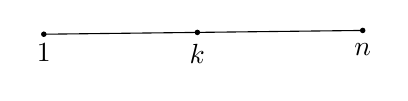
\begin{tikzpicture}[x=.75cm,y=.6cm]
\draw (0,0)--(5.4,.08);
\foreach \x/\lab in {0/1,2.6/k,5.4/n}{\fill (\x,.08*\x/5.4) circle(1pt);\node[below] at (\x,0) {$\lab$};}
\end{tikzpicture}}

\[
M=\prod_{1\le i\le n}C'_i\qquad
C'_i=\begin{cases}
C_i&\text{si }i\in J'\\
C_j&\text{si }j\in J''\\
C_{j+1}&\text{si }j\in\unsure{\complement J'|\complement J''}\ \unsure{J''}
\end{cases}
\]

\[
\begin{aligned}
\delta_n(B_0,\ldots,B_{n})&=
 B_0^n B_1^{n-1}\ldots B_{n-1}^{1}\underbrace{L_n(B_1,\ldots,B_{n-1})}_{\text{polynôme \deleted{\unsure{homogène de degré $[n/2]$}}}}
 \deleted{\unsure{\text{degré}}}
\end{aligned}
\]
\margin{Attention, \unsure{pas 0|$p\to0$|$p\geq0$}!} $C'_i$ contient en facteur $B_k$ \deleted{\unsure{(et ce facteur}} à la puiss. 1 exactement) sss \deleted{\unsure{entier}} $i\ge k$, \uline{ou} $i=k-1$ \uline{et} $i\in J^{\unsure{'''|''}}$ i.e. $k\in J''$

\[
\begin{aligned}
L_n(B_1,\ldots,B_{n-1})
&=\sum_{0\le p\le[n/2]}(-1)^p2^{n-2p}
\sum_{\substack{\deleted{\unsure{\text{suites de }p\,J_i}}\\J\in\mathcal P_p([1,n-1])\\J\text{ ne contient pas 2}\\\text{entiers consécutifs}}} B_J\\
&=2^n\unsure{-|+}2^{n-2}\sum_{\unsure{1|0}\le i\le n-1}B_i
+2^{n-4}\sum_{\substack{1\le i<j\le n-1\\j\ne i+1}}B_iB_j\\
&\quad-2^{n-6}\sum_{\substack{1\le i<j<k\le n\\\vdots\quad\vdots}}B_iB_jB_k+\ldots
\end{aligned}
\]
\margin{\unsure{Attention|les}, \unsure{$n-1$ et non $n$|non circulaire} !}
% archive sheet number: 48
\scanpage{50}
\[
\deleted{\Pi_p(B_1,\ldots,B_n)=\sum_{J\in\mathcal P_p[1,n]}}\qquad B_i=B'_i+4
\]

\[
\begin{aligned}
\deleted{\unsure{\sum|\Sigma}}\quad B'_1B'_2&=B'_2B'_3\ldots=B'_nB'_{n+1}=0\\
(2-\tfrac{B_1}{2})(2-\tfrac{B_2}{2})\ldots(2-\tfrac{B_n}{2})&=\frac{(-1)^n}{2^{n}}.
\end{aligned}
\]

\[
\begin{aligned}
L_1&=2\qquad L'_1=1\\
L_2&=4-(B_1\deleted{\unsure{+B_2}})=\deleted{\unsure{4-(\alpha_0+\alpha_1)}\ (\alpha_0+{}}2-\alpha_1=-(\alpha_1-2)\\
L_3&=8-2(B_1+B_2)\deleted{\unsure{+B_3}})=-2\bigl[\unsure{(}\alpha_1+\alpha_2)\deleted{\unsure{+2+2}}\bigr]\\
L_4&=\underbrace{16-4(B_1+B_2+B_3\deleted{\unsure{+B_4}})+\bigl(\sum_{1\le i\unsure{\le|<}j\le3}B_iB_j}_{\phantom{16}}
-(B_1B_2+B_2B_3+B_3B_4)
\end{aligned}
\]

\[
\begin{aligned}
&\deleted{(2-\tfrac{B_1}{\unsure{2|1}})(2-\tfrac{B_2}{2})}\\
&-4(\alpha_1+\alpha_2+\alpha_3+\deleted{\unsure{\alpha_4}})-\unsure{8}+ \bigl[\deleted{(\alpha_0+2)(\alpha_1+2)}+(\alpha_0+2)(\alpha_2+2)+\deleted{\unsure{(\alpha_0+2)(\alpha_3+2)}}\\
&\hspace{17em}+\deleted{\unsure{(\alpha_1+2)(\alpha_3+2)}}\bigr]\\
&\deleted{=-4-4(\alpha_0+\alpha_1+\alpha_2\unsure{+\alpha_3})+2(\alpha_0+\alpha_2+\alpha_0+\alpha_3+\alpha_1+\alpha_3)+\alpha_0\alpha_2+\alpha_0\alpha_3}+\alpha_1\alpha_3\\
&\hspace{16em}\deleted{\unsure{2\alpha_0+2\alpha_2+\alpha_2+2\alpha_3|2\alpha_0+2\alpha_1+\alpha_2+2\alpha_3}}\\
&=-4-2(\alpha_1+\inserted{2\alpha_2+}\alpha_3)+(\alpha_1\alpha_3\deleted{\unsure{+\alpha_0\alpha_2+\alpha_0\alpha_3}})=(\alpha_1-2)(\alpha_3-2)\unsure{-|+}4(\alpha_2+2)
\end{aligned}
\]

\uline{NB} $L_{n-1}(B_1,\ldots,B_{n-1})=L_{n-1}(B_{n-1},\ldots,B_1)$

\begin{center}\rule{2.5cm}{0.35pt}\end{center}

\[
\begin{aligned}
\det\left(\begin{array}{cccccc}
2\deleted{\unsure{c_0}}&-c_0&0&&&\\
-c_0&2c_0&-c_1&0&&\\
0&-c_1&2c_1&&&\\
0&0&-c_2&\ddots&&0\\
&&&&c_{\unsure{n-2|n-1|n-3}}&-c_{n-1}\\
&\ldots&&0&-c_{n-1}&2c_{n-1}
\end{array}\right)_{\leftrightarrow\,\substack{\deleted{\unsure{\text{ordre }n}}\\\text{ordre }n+1}}
&=\Delta_{n+1}(\underbrace{1,c_0,\ldots,c_{n-1}}_{n+1\ \text{arg}})=2\Delta_n(c_0,\ldots,c_{n-1})\\
&\hspace{7em}-c_0^2\Delta_{n-1}(c_1,\ldots,c_{n-1})
\end{aligned}
\]

\[
\begin{aligned}
&=\delta_{n+1}(1,B_0,\ldots,B_{n-1})=B_0^n B_1^{n-1}\ldots B_{n-1}L_{n+1}(\deleted{\unsure{1,}}B_0,\ldots,B_{n-1})\\
&\deleted{\unsure{L_2}\delta_{n+1}(1,B_0)=B_{\unsure{n|0}}\ldots}
\qquad \deleted{\begin{aligned}L_2(1,B_0)&=4-{}\\ L_3(1,B_0,&\end{aligned}}\\
&\delta_2(1,B_0)\deleted{\unsure{B_1}}=B_0 L_2(1,B_0)=B_0(4-B_0)=-(\alpha_0+2)(\alpha_0-2)=4-\alpha_0^2\\
&\delta'_3(1,B_0,B_1)=B_0^2B_1L'_3(\deleted{\unsure{1,}}B_0,B_1)=\deleted{\unsure{B_0^2B_1(4}}-B_0^2B_1(\alpha_0+\unsure{\alpha_2|\alpha_1})\\
&\delta_4(1,B_0,B_1,B_2)=B_0^3B_1^2B_2\underbrace{L_4(B_0,B_1,B_2)}_{(\alpha_0-2)(\alpha_2-2)-4(\alpha_1+2)}
\end{aligned}
\]

\deleted{$\begin{aligned}
\det\begin{pmatrix}2c_0&-c_1\\-c_1&2c_1\end{pmatrix}
&=4c_0c_1-c_1^2=\\
&=c_1(4c_0-c_1)\\
&=B_0^2B_1(4-B_1)
\end{aligned}$}
% archive sheet number: 49
